\section{Event and Object Selection}
\label{sec:AN_Selection}

%In this chapter we document the electron, muon, and photon identification and isolation criteria, $E_T^{MET}$ criteria, and provide the results of comparing simulation with data.
\subsection{Object Selection}
\label{sec:AN_ObjectSelection}

We select events with a muon and a photon in the final state for the muon channel and events with an electron and a photon in the final state for the electron channel. 

We apply selection requirements on transverse momenta of $P_T^{\mu}>25$ GeV on muons,  $P_T^e>30$~GeV on electrons and $P_T^{\gamma}>15$~GeV on photons. In addition, electrons and photons must be within barrel (EB) or endcap (EE) sections of the Ecal which corresponds to pseudorapidity ranges of $|\eta^{e,\gamma}| < 1.4442$ and $1.566 < |\eta^{e,\gamma}| < 2.5$, respectively. Muons must be within $|\eta^{\mu}|<2.1$. Selection requirements on $P_T^{\mu}$, $\eta^{\mu}$, and $P_T^e$ are determined by the trigger requirements, $\eta^{e,\gamma}$ criteria are determined by the geometrical limitations of the detector acceptance, and $P_T^{\gamma}>15$~GeV is the phase space requirement.

CMS Particle Object Group (POG) provides their recommendations for object identification~(ID) criteria for any given period of data collection. To satisfy a muon~ID criteria, objects, first of all, must be reconstructed as muons by the PF algorithm. Quality requirements are applied on tracks reconstructed in both the tracking system and the muon system. These two tracks must match. An isolation from the other nearby PF objects is also required.

%Recommendations for~2012 data include two sets of muon~ID criteria: ``Tight'' and ``Loose'', and four sets of electron and photon~ID criteria: ``Tight'', ``Medium'', ``Loose'' and ``Veto''. 

% Muon ID
% https://twiki.cern.ch/twiki/bin/view/CMSPublic/SWGuideMuonId#Tight_Muon

% Electron ID
% https://twiki.cern.ch/twiki/bin/viewauth/CMS/EgammaCutBasedIdentification
% Photon ID
% https://twiki.cern.ch/twiki/bin/viewauth/CMS/CutBasedPhotonID2012
The electron~ID and photon~ID criteria include requirements on the shower shape, on ratio of energies releazed in ECal and HCal. The electron~ID also includes requirements on the track quality. Similarly to muons, electrons and photons must be isolated from the nearby PF objects. For the photon~ID, the isolation consists on three parts: charged hadron, neutral hadron, and photon isolation. To reject electron reconstructed as photons, ``conversion safe electron veto'' (CSEV) is recommended as a part of any photon~ID.

% [Almost] QUOTE from Wgg AN:
%A conversion save electron veto (CSEV) CSEV rejects photons that have an associated track that is not identified as resulting from a converted photon. Pixel seed veto (PSV) requires that there is no track seed identified in the pixel detector from back-propagating from the measured supercluster. This cut removes some conversion photons, but also reduces the background from electron.

%For the muon and electron selection, we apply ``Tight''~ID criteria. For photon selection, we apply ``Medium''~ID criteria

In $W\gamma$ measurement, we applied object~ID criteria as recommended by POG with one exception: in the electron channel, the CSEV is substituted with the ``pixel seed veto'' (PSV) as recommended by CMS $W\gamma\gamma \rightarrow l\nu\gamma\gamma$ measurement team~\cite{ref_Wgg8TeV}. CSEV rejects photons with associated track originated from a converted photon. Such tracks are not identified, thus, such particle is reconstracted as a photon rather than an electron. But some of such tracks can originate from real electrons, and by requiring CSEV, we reject this background. PSV rejects photons that have any track seed in the pixel detector that can match to the measured ECal supercluster. PSV is tighter requirement that CSEV and, therefore, is used in the electron channel only where we have much larger background from electrons misidentified as photons. %No restrictions on the maximum number of the final state photons are applied, however, 

To reduce backgrounds from the process with two or more leptons, such as $Z\gamma\rightarrow l l \gamma$ process, in the muon channel, we reject all events that have the second reconstructed muon candidate with $P_T^{\mu}>10$~GeV and $|\eta|^{\mu}<2.4$, and, in the electron channel, we reject events that have the second reconstructed electron candidate with $p_T^e>10$~GeV and satisfying the ``Veto''~ID criteria.

% SCALE FACTORS MAY MOVE TO ACCxEFF CHAPTER
Selection criteria are applied on the data sample as well as on all MC samples. The selection efficiency may differ between data and MC. The ratios between data and MC efficiencies are called the scale factors (SF). The SF for the selection criteria recommended are provided by CMS POG. For the PSV criterion in the photon selection in the electron channel, additional SF are applied as derived by the $W\gamma\gamma$ team~\cite{ref_Wgg8TeV}. All SF are listed in App.~\ref{sec:SFsTables}.

\subsection{Event Level Selection}
\label{sec:AN_Selection_EventLevel}

In the final state of the $W\gamma\rightarrow l\nu\gamma$ process, there is a lepton, a photon, and a neutrino. Because of that, we select events with exactly one lepton (muon or electron), a photon, both originating from the primary vertex, and with the significant missing transverse energy $E_T^{miss}$. The selection criteria for the individual electrons, muons and photons are described in Ch.~\ref{sec:AN_ObjectSelection}.

The standard tool to detec a particle that decays is to reconstruct its invariant mass out of its decay products. Decay products of a $W$ boson are a charged lepton and a neutrino. CMS does not detect neutrino, it only measures the missing momentum in the plane, transverse to the beamline, which can be partially associated with a neutrino. The transverse momentum is described by two parameters: $E_T^{miss}$ and $\phi^{miss}$. Because we do not have an estimate of the longitudial component of a neutrino, we cannot construct an invariant mass of a $W$~boson. Instead, we construct its transverse mass:
\begin{equation}
M_T^W=\sqrt{(2  P_T^{l}  E_T^{miss}  (1-\cos{(\phi^{l}-\phi^{miss})}))},
\end{equation}
\noindent{where $P_T^l$ is a lepton transverse momentum, $\phi^{l}$ is an azimuthal angle of the lepton momentum, and $\phi^{miss}$ is an azimuthal angle of the missing transverse momentum. To enchance contribution from $W\gamma$ compared to background processes without a final state neutrino, we require $M_T^W>40$~GeV. Value of $40$~GeV was recommended by the CMS Standard Model Physics (SMP) group because the same requirement was used in $W\gamma\gamma$ measurement. The $M_T^W$ distribution is shown in Fig.~\ref{fig:DATAvsMC_WMt}. Photons with $P_T^{\gamma}<45$~GeV are selected for this plot because for such photons we do not expect them to be result of a new physics process.}

After the listed selection criteria are applied, significant background from DY+jets in the electron channel remains. This background is caused by one of the electrons misidentified as a photon. Its contribution is the most significant around the invariant mass of the electron-photon system $M_{e\gamma}$ close to the mass of the $Z$ boson (Fig.~\ref{fig:DATAvsMC_Mpholep1})because the distribution of $M_{ee}$ in the $Z\rightarrow e e$ decay is peaking at the value of the Z boson mass. To reduce this background, we apply $Z$-mass window selection criterion, more specifically, events with $70$~GeV$<M_{e\gamma}<110$~GeV are rejected. 

In addition to $W\gamma$-selected datasets, we also prepare $Z\gamma$-selected datasets in muon and electron channels. Selection requirements include at least two muons (or electrons) and at least one photon in the final state. Kinematis and identification requirements on the objects are the same as for the $W\gamma$ selection. Unlike in $W\gamma$, in $Z\gamma$ selection in the electron channel, photons are required to pass ``Medium'' ID without any modifications. Invariant mass of the final state lepton pair is required to be $M_{ll}>50$~GeV. Finally, a separation between photon and each lepton must be $\Delta R>0.7$.

Finally, the separation $\Delta R=\sqrt{({\Delta\phi}^2+{\Delta\eta}^2)}$ between the final state lepton and photon is required to be $\Delta R(l,\gamma)>0.7$ to enhance the TGC contribution. In case if there is more than one photon in the selected event, the candidate with the photon of the highest~$P_T^{\gamma}$ is selected. 

In addition to $W\gamma$-selected datasets, we also prepare $Z\gamma$-selected datasets in muon and electron channels. Selection requirements include at least two muons (or electrons) and at least one photon in the final state. Kinematis and identification requirements on the objects are the same as for the $W\gamma$ selection. Unlike in $W\gamma$, in $Z\gamma$ selection in the electron channel, photons are required to pass ``Medium'' ID without any modifications. Invariant mass of the final state lepton pair is required to be $M_{ll}>50$~GeV. Finally, a separation between photon and each lepton is required to be the same as in the $W\gamma$ selection: $\Delta R>0.7$. 

\subsection{Selected Events}

After the selection procedure, 175889 and 85643 events survived in the muon and electron channels, respectively. These events are used for the total and differential cross setion measurements with respect to $P_T^{\gamma}$. Distributions of $P_T^{\gamma}$ of the selected events are shown in Fig.~\ref{fig:DATAvsMC} and documented in Tab.~\ref{tab:yields_Wg_to_munu_}-\ref{tab:yields_Wg_to_enu_}. The plots and tables include information about the underflow $P_T^{\gamma}$ bin ($10-15$~GeV). The measurement in this bin is used for the detector resolution unfolding (Ch.~\ref{sec:Unfolding}). 

Selected samples are dominated by $W$+jets events. The main mechanism of a jet to be misidentified as a photon is a $\pi^0 \rightarrow \gamma\gamma$ decay. Photon~ID requirements rejects most of such fragmentation photons, however, a $W$+jets event has much larger probability to be produced in a $pp$ collision than a $W\gamma$ event, and, therefore, even a small fraction of fragmentation photons from $W$+jets events becomes a significant background to $W\gamma$.  

There are large discrepancies between data and MC predictions in all the distributions as shown in Fig.~\ref{fig:DATAvsMC_WMt}-\ref{fig:DATAvsMC}. Possible reasons for the discrepancies include but are not limited to uncerntainties in the normalizations of all MC samples involved and difficulties in modeling jet fragmentation. Therefore, the data-driven background estimates are necessary (Ch.~\ref{sec:BackgroundSubtraction}).

\begin{figure}[htb]
  \begin{center}
   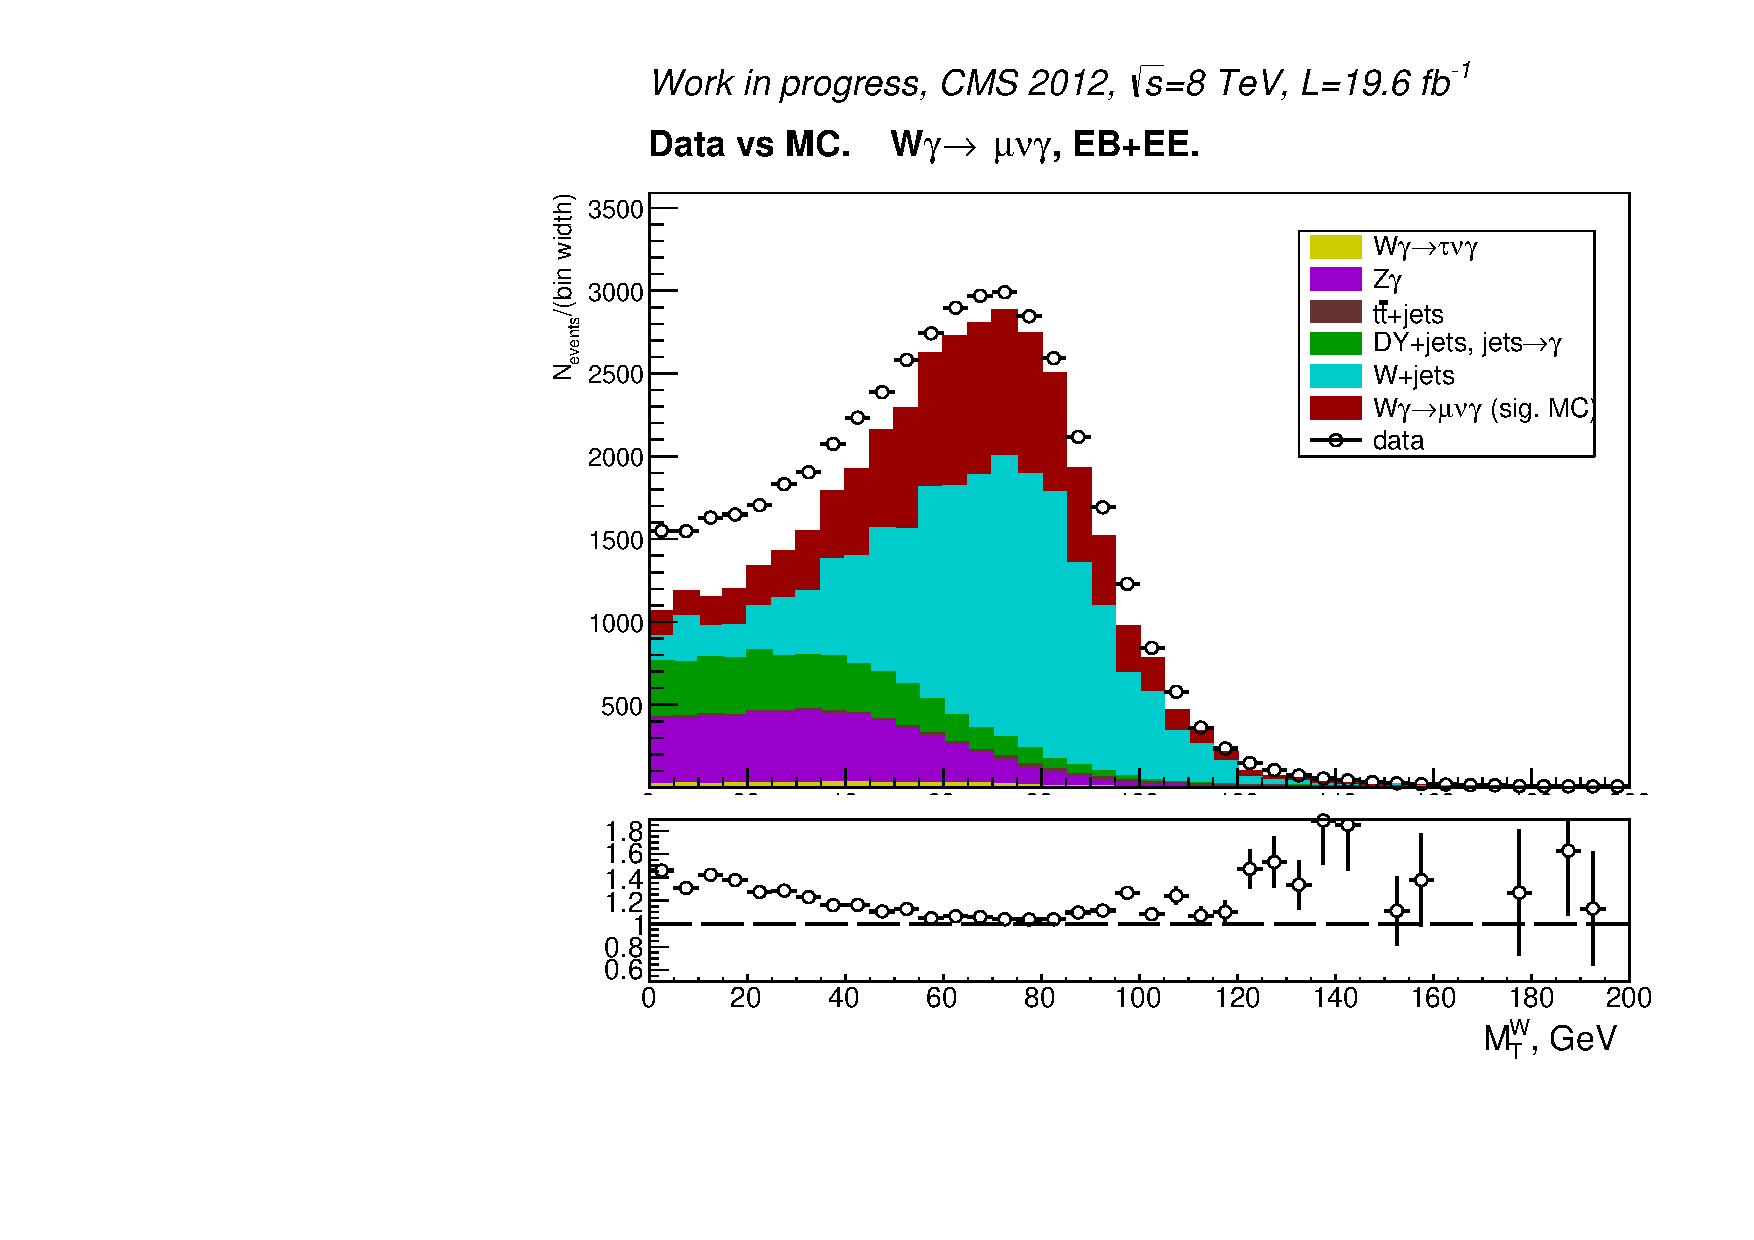
\includegraphics[width=0.5\textwidth]{../figs/figs_v11/MUON_WGamma/PrepareYields/c_TotalDATAvsMC_EtaCommon__WMtVERY_PRELIMINARY.pdf}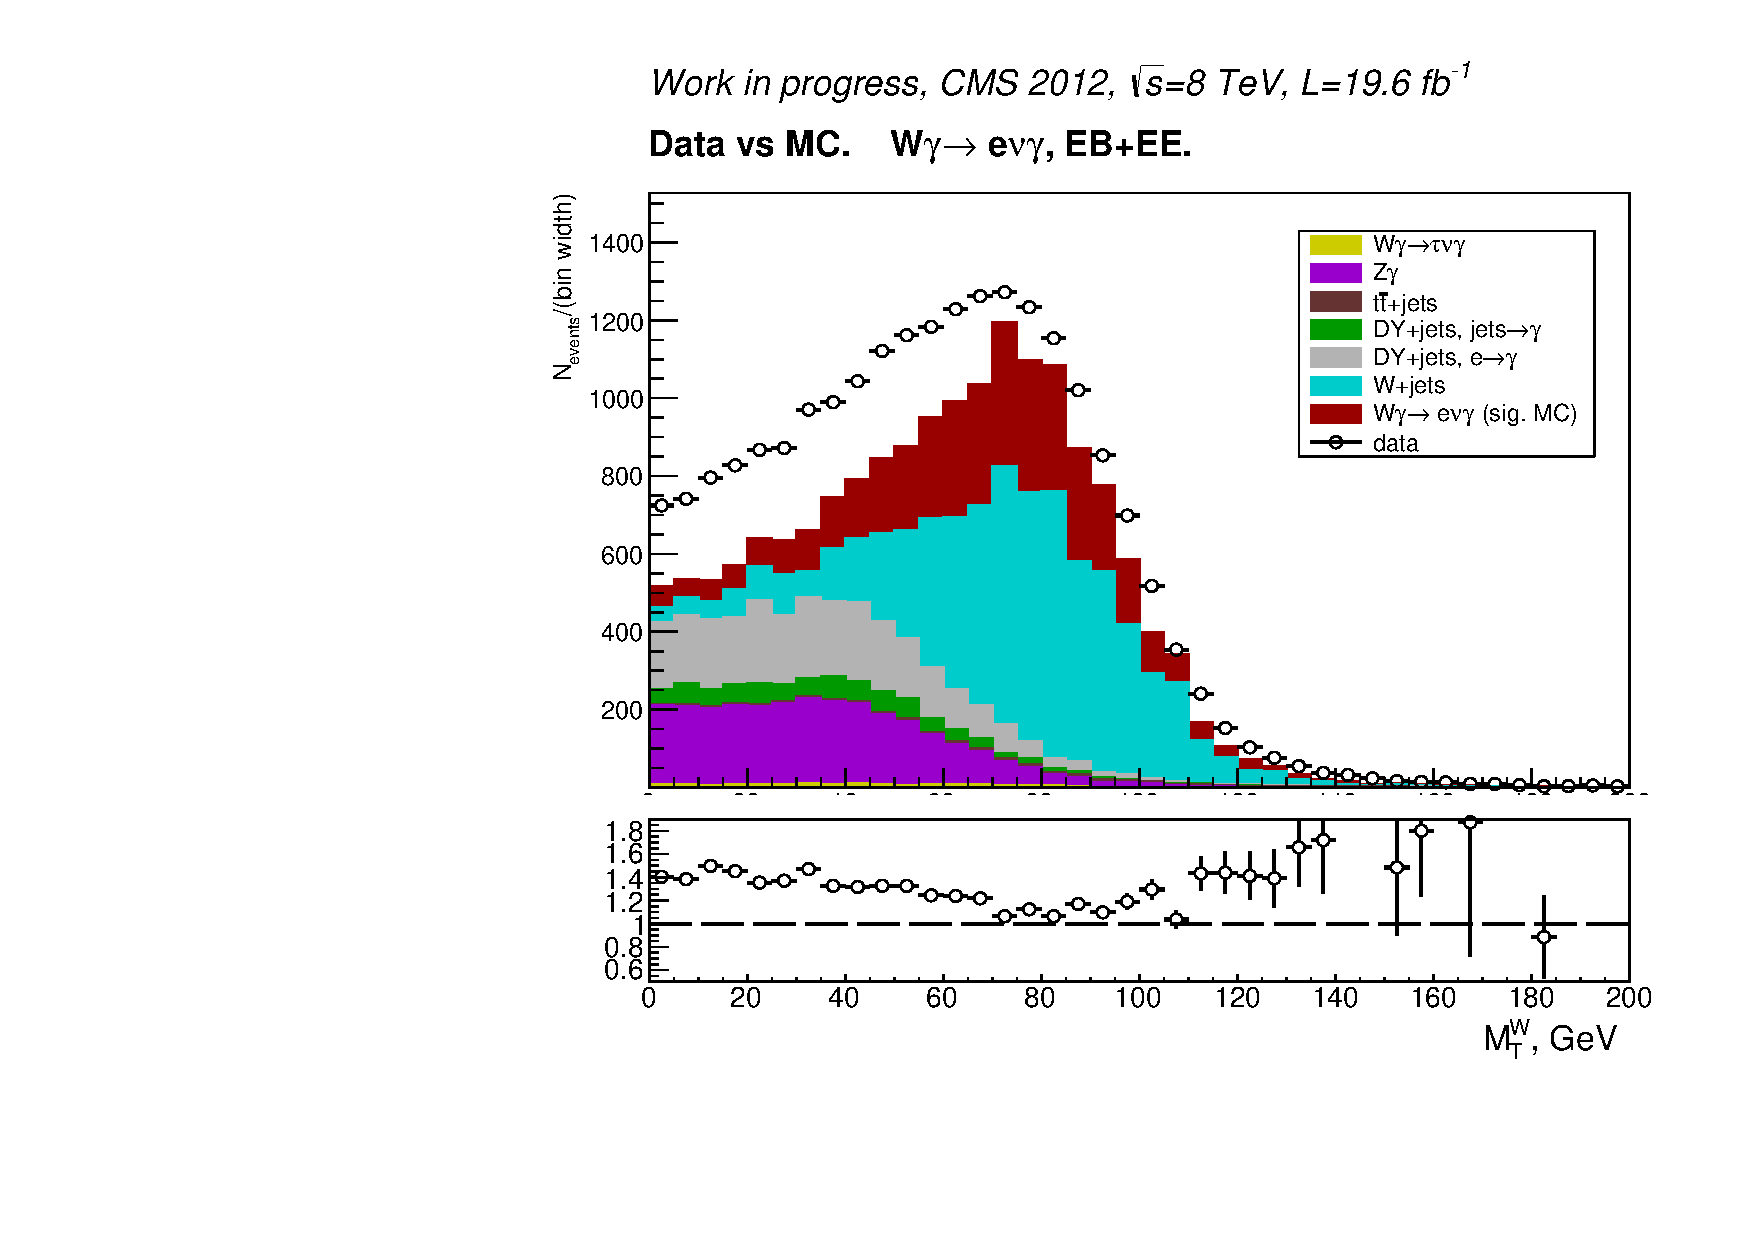
\includegraphics[width=0.5\textwidth]{../figs/figs_v11/ELECTRON_WGamma/PrepareYields/c_TotalDATAvsMC_EtaCommon__WMtVERY_PRELIMINARY.pdf}
  \caption{ $M_T^W$ distribution of $W\gamma$ candidates. Data vs MC plots. Left: muon channel, right: electron channel. All selection criteria except $M_{T}^W$ requirement are applied on these plots. $15$~GeV$<P_T^{\gamma}<45$~GeV. }
  \label{fig:DATAvsMC_WMt}
  \end{center}
\end{figure}

\begin{figure}[htb]
  \begin{center}
   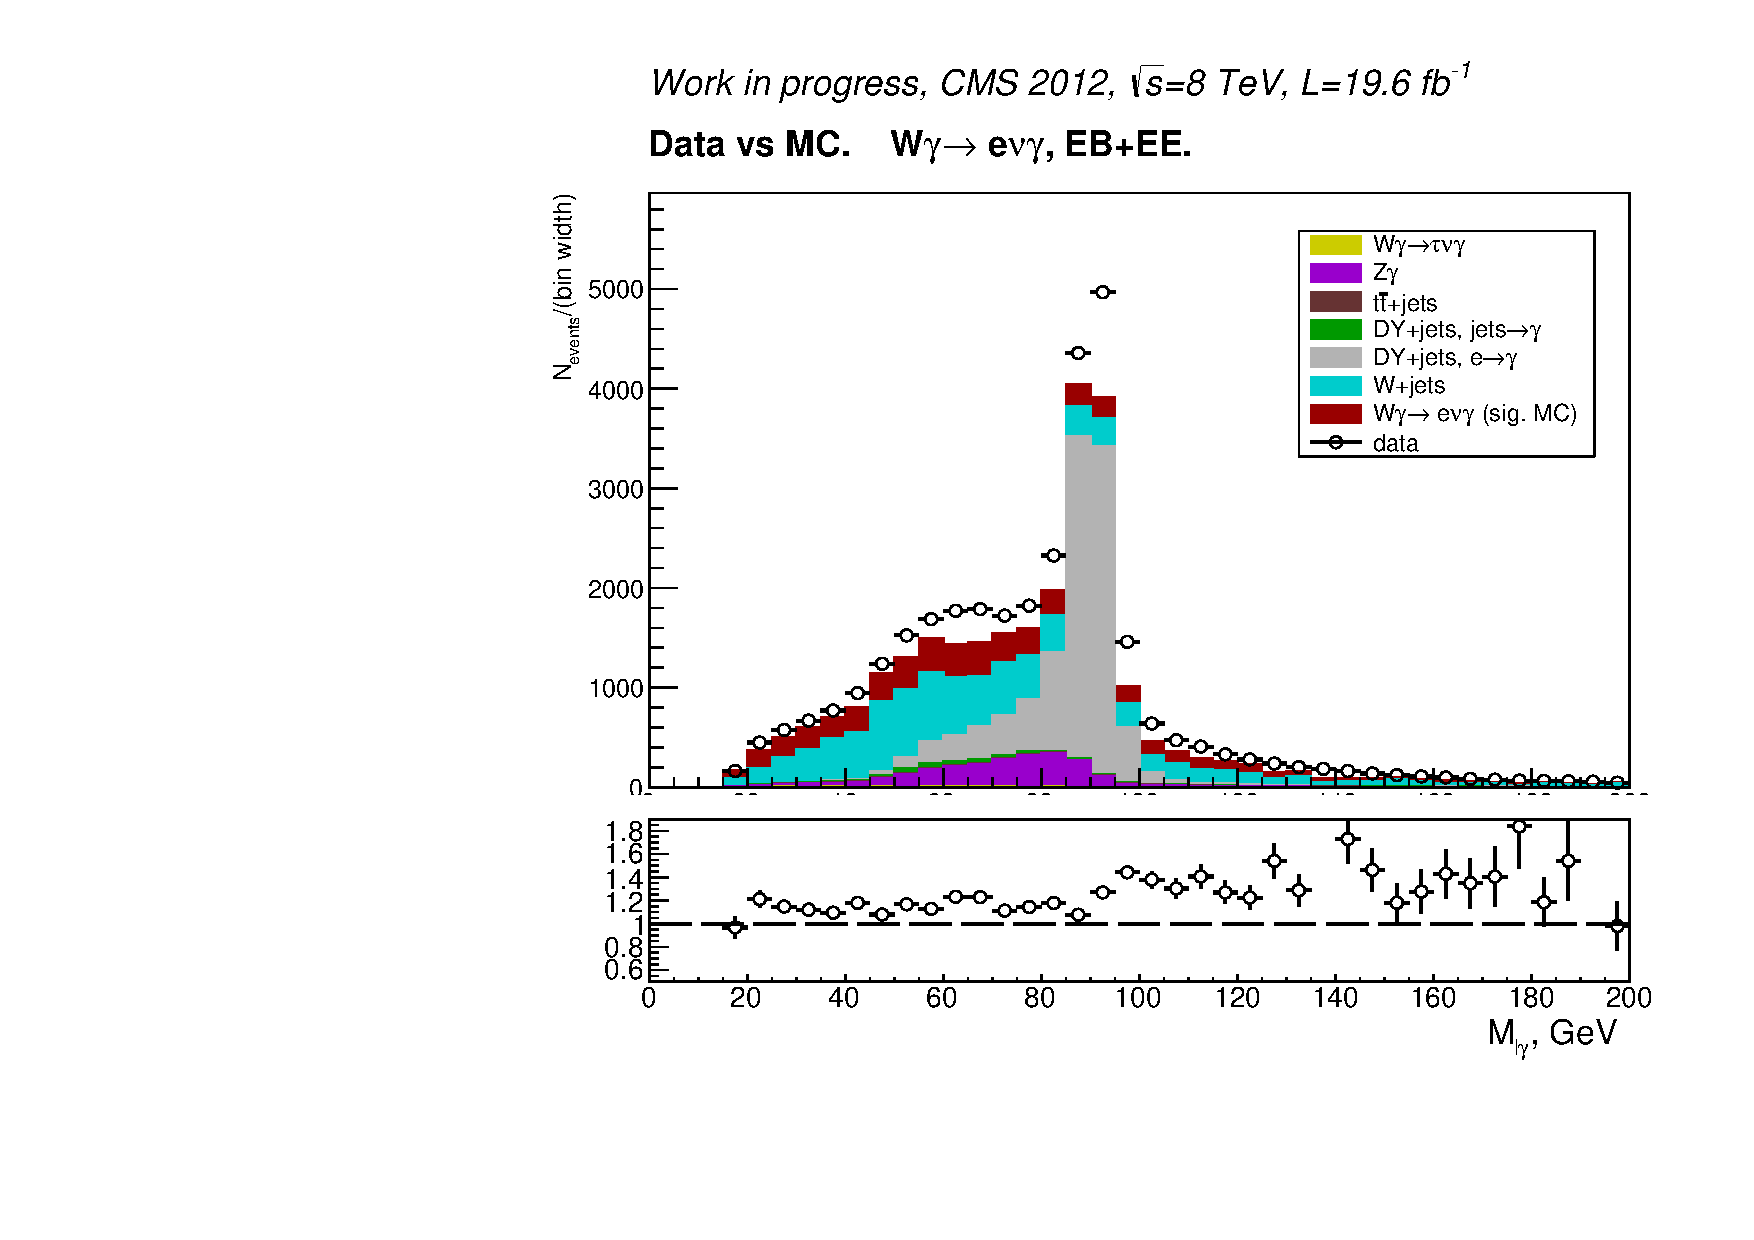
\includegraphics[width=0.65\textwidth]{../figs/figs_v11/ELECTRON_WGamma/PrepareYields/c_TotalDATAvsMC_EtaCommon__Mpholep1PRELIMINARY_FOR_E_TO_GAMMA_WITH_PSV_CUT.pdf}
  \caption{$M_{l\gamma}$ distribution of $W\gamma$ candidates in the electron channel. Data vs MC plots. All selection criteria except $Z$-mass window are applied on this plot. $P_T^{\gamma}>15$~GeV. }
  \label{fig:DATAvsMC_Mpholep1}
  \end{center}
\end{figure}

\begin{figure}[htb]
  \begin{center}
   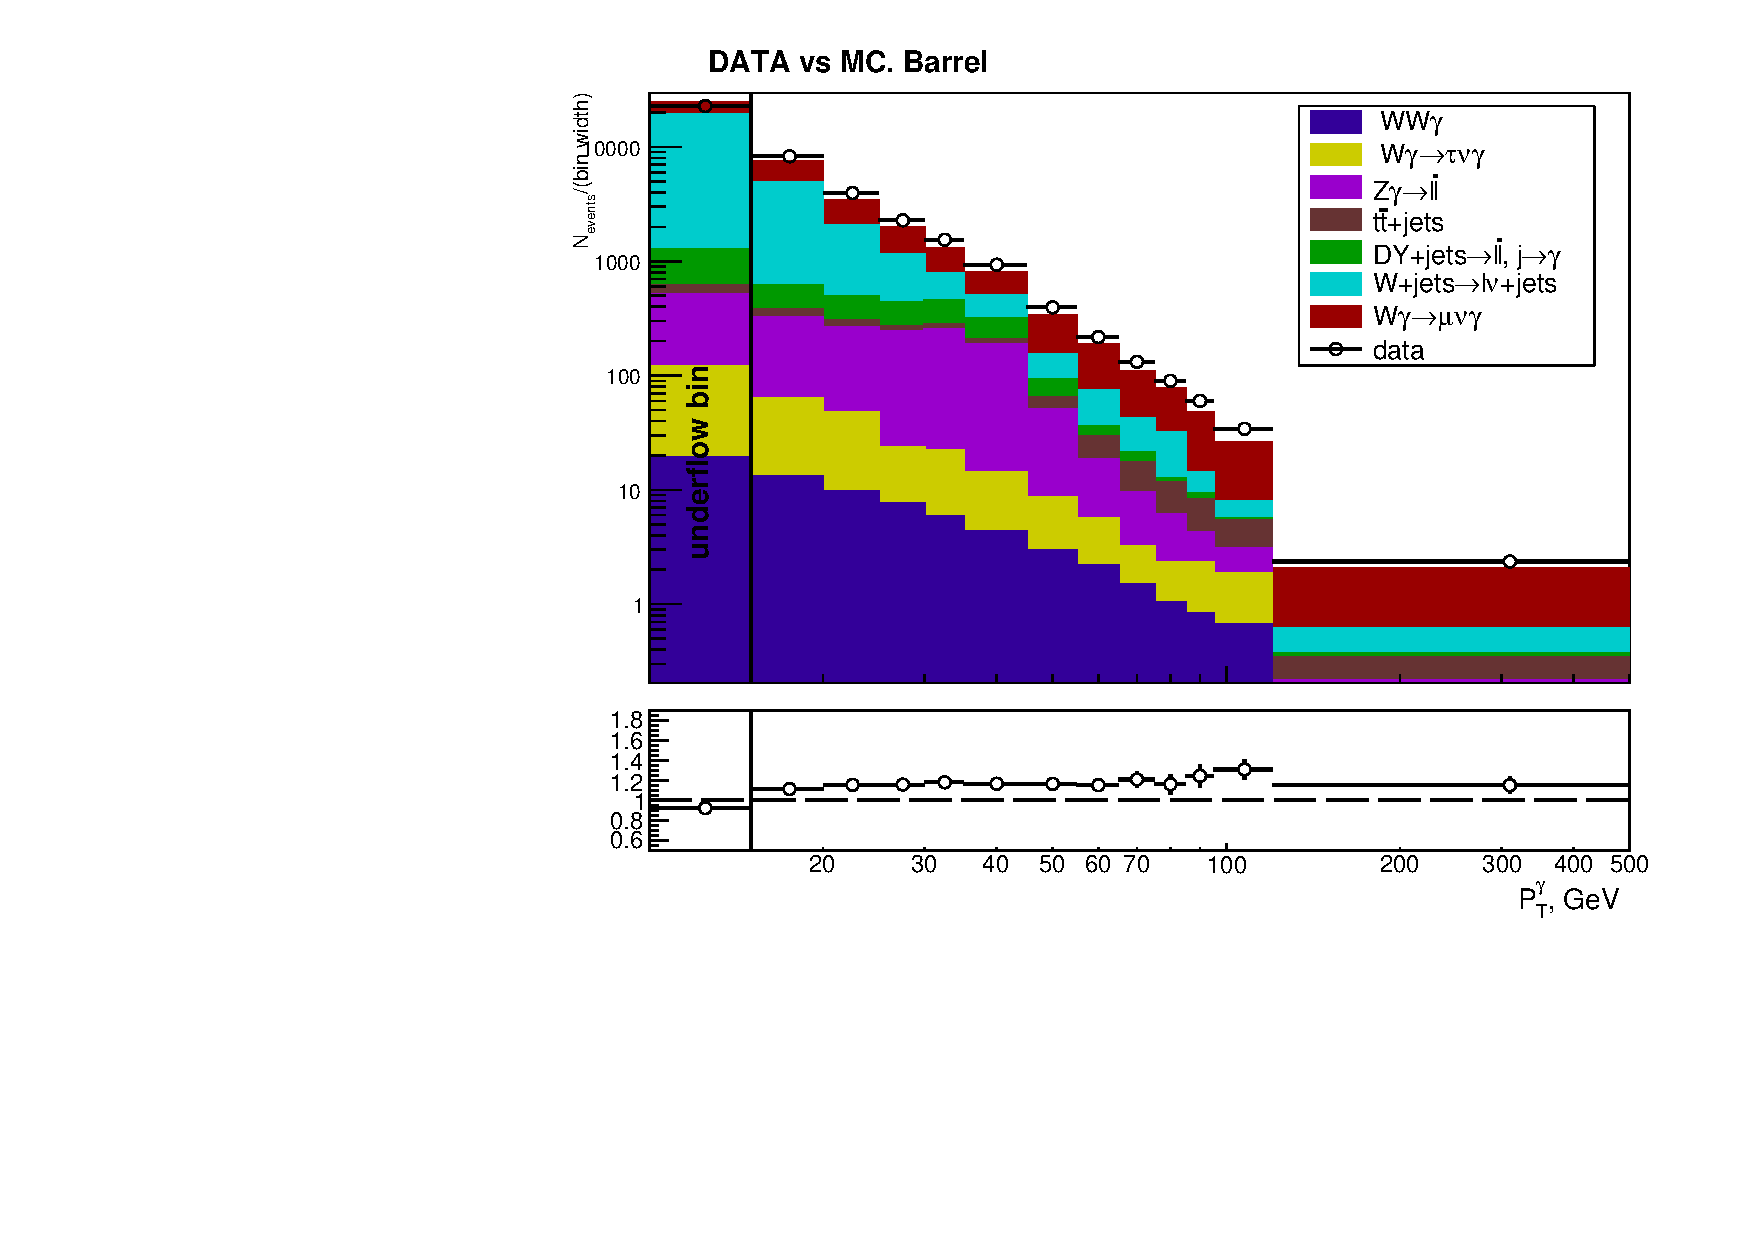
\includegraphics[width=0.45\textwidth]{../figs/figs_v11/MUON_WGamma/PrepareYields/c_TotalDATAvsMC_Barrel__phoEt.pdf}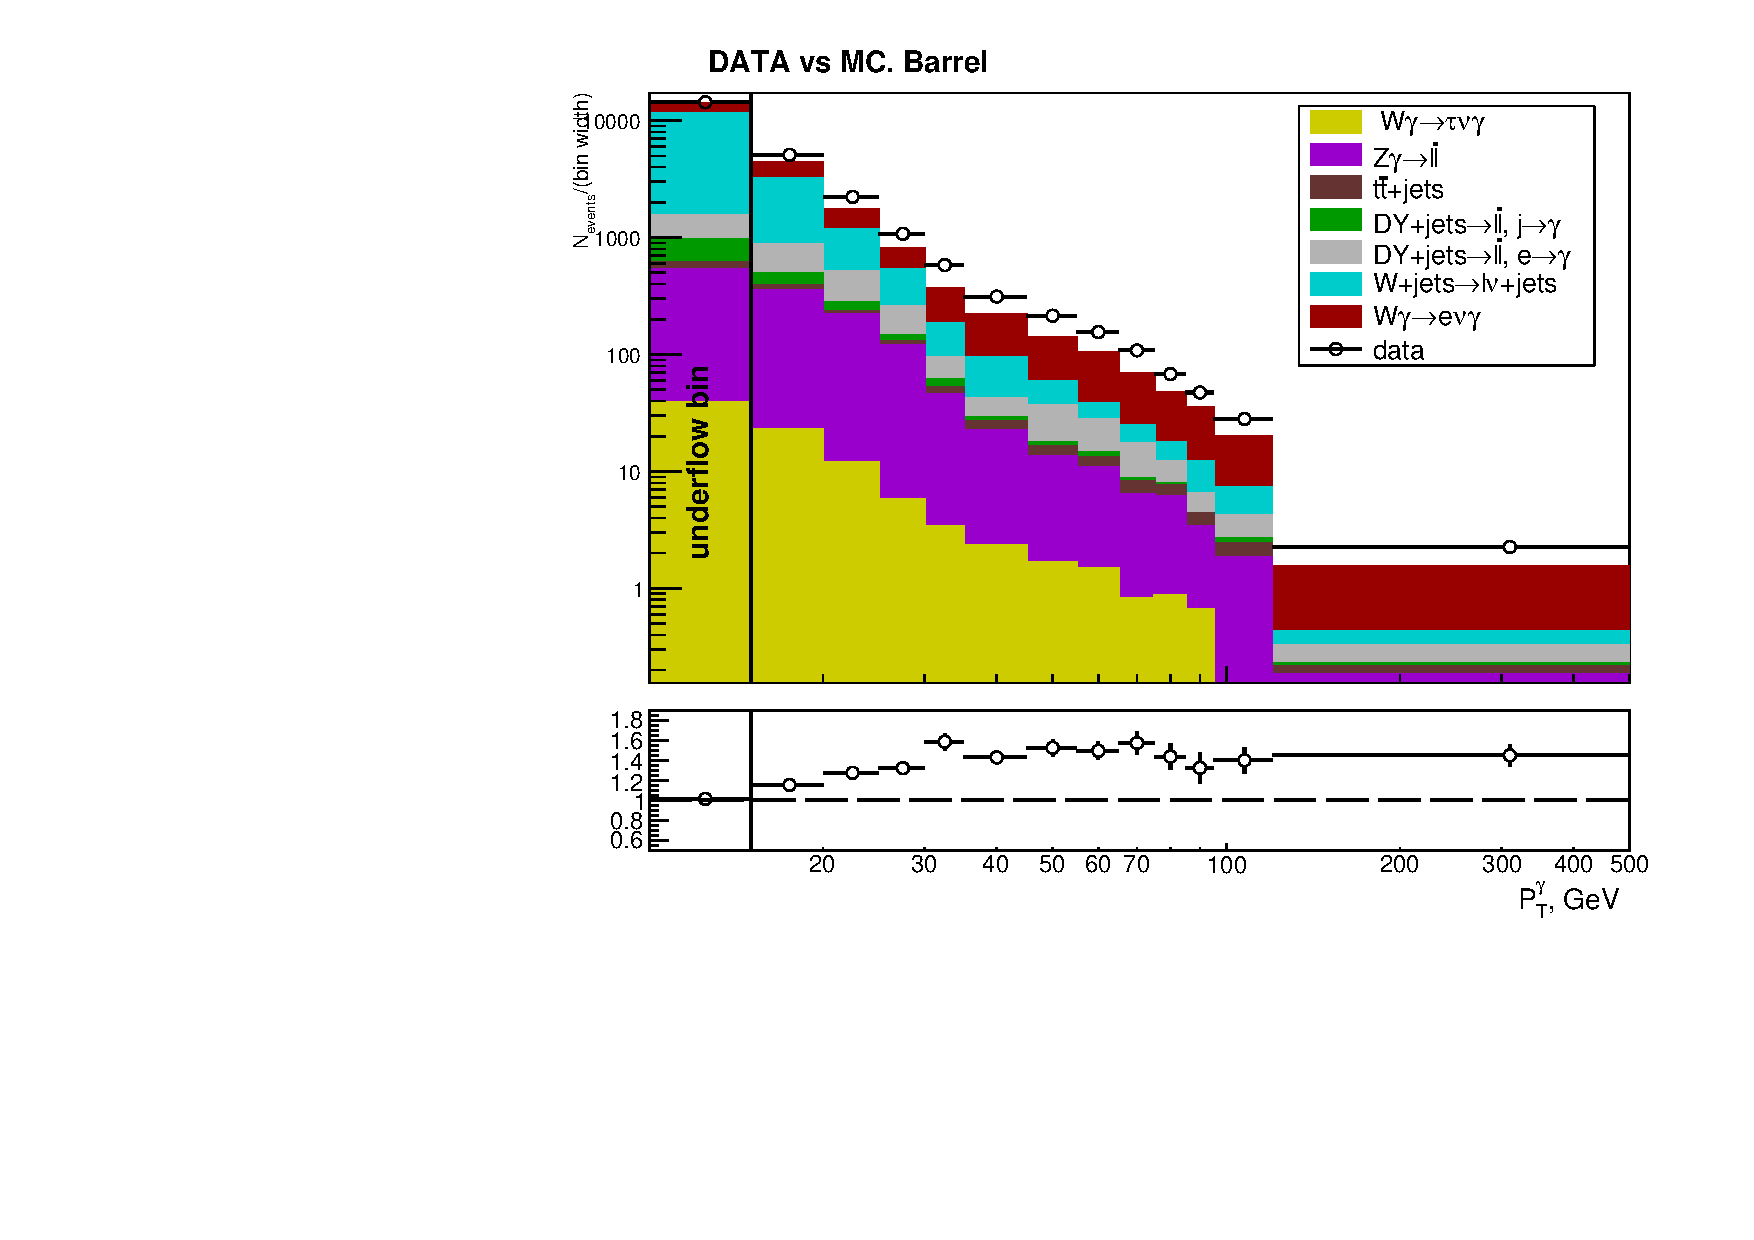
\includegraphics[width=0.45\textwidth]{../figs/figs_v11/ELECTRON_WGamma/PrepareYields/c_TotalDATAvsMC_Barrel__phoEt.pdf}
   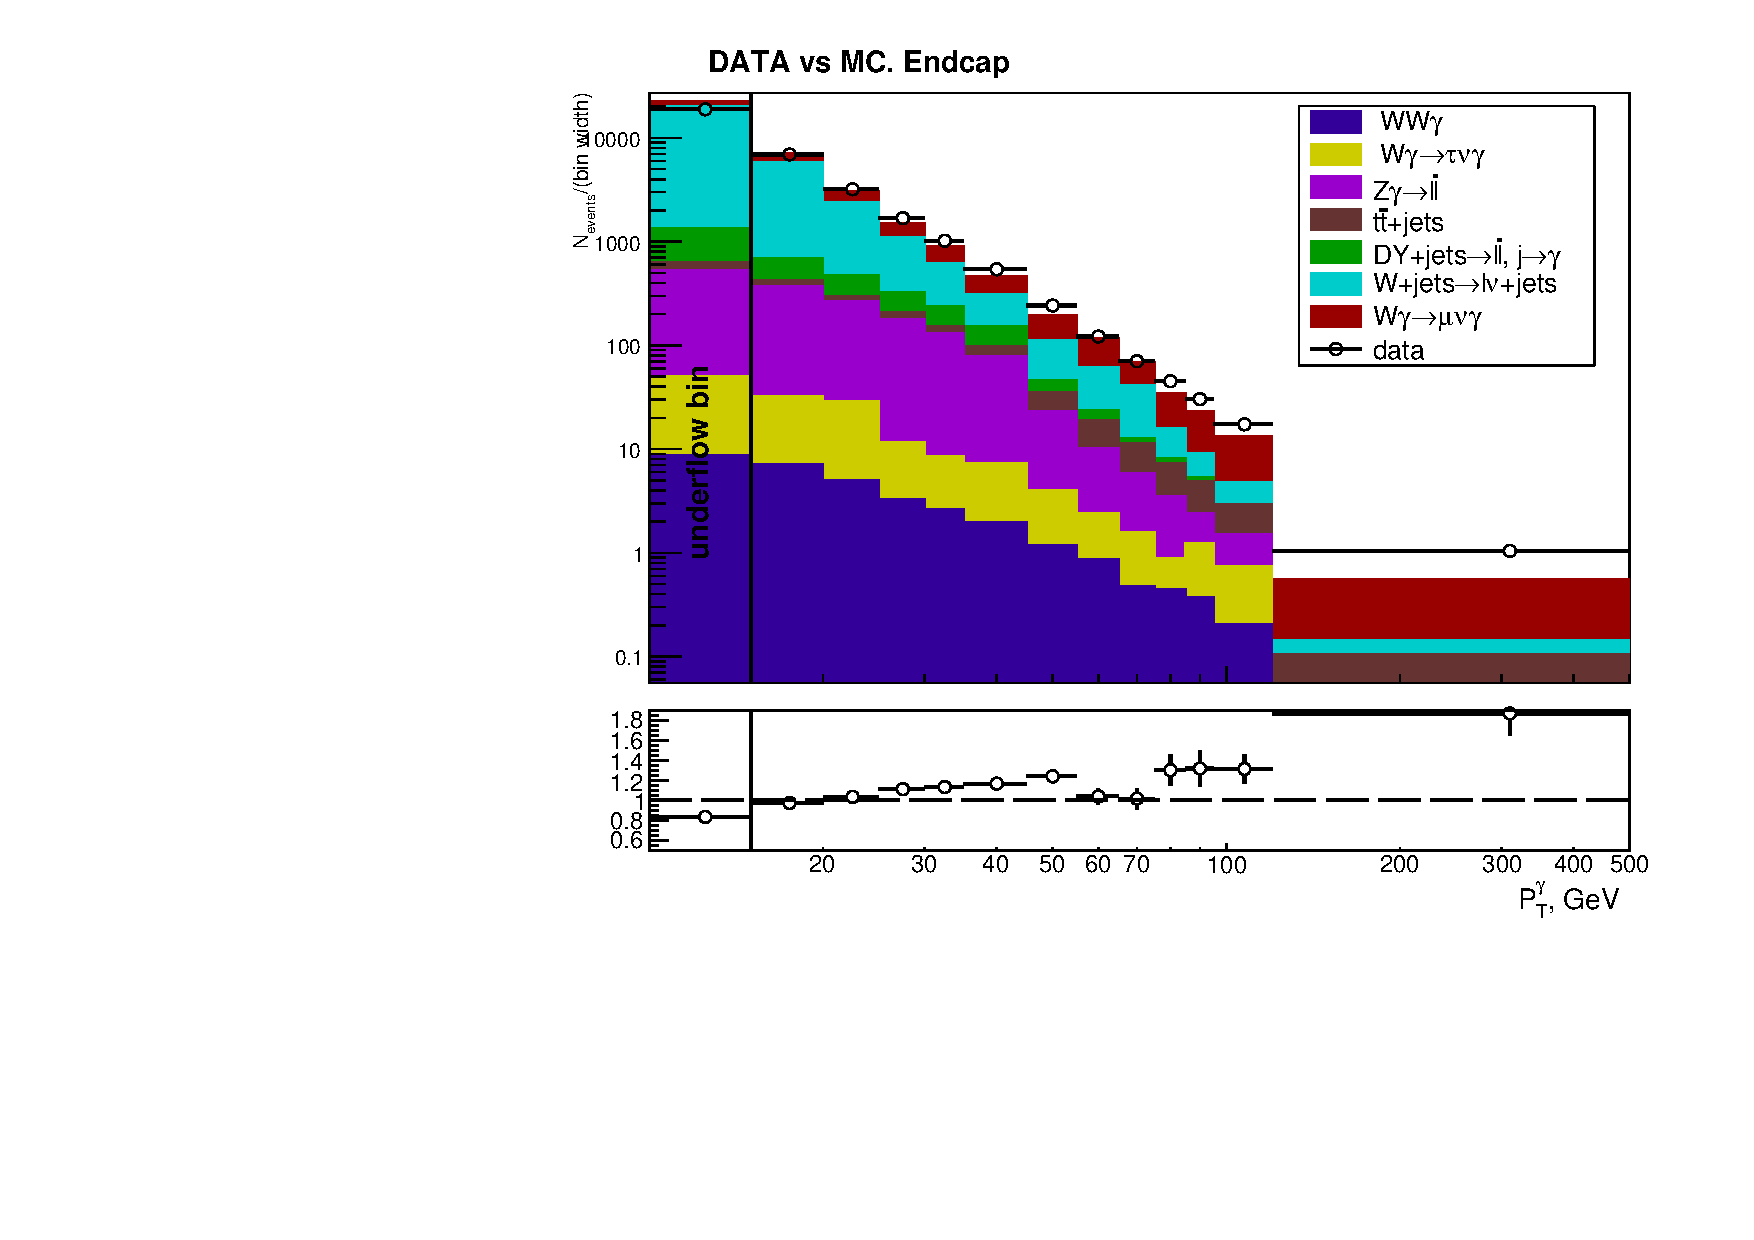
\includegraphics[width=0.45\textwidth]{../figs/figs_v11/MUON_WGamma/PrepareYields/c_TotalDATAvsMC_Endcap__phoEt.pdf}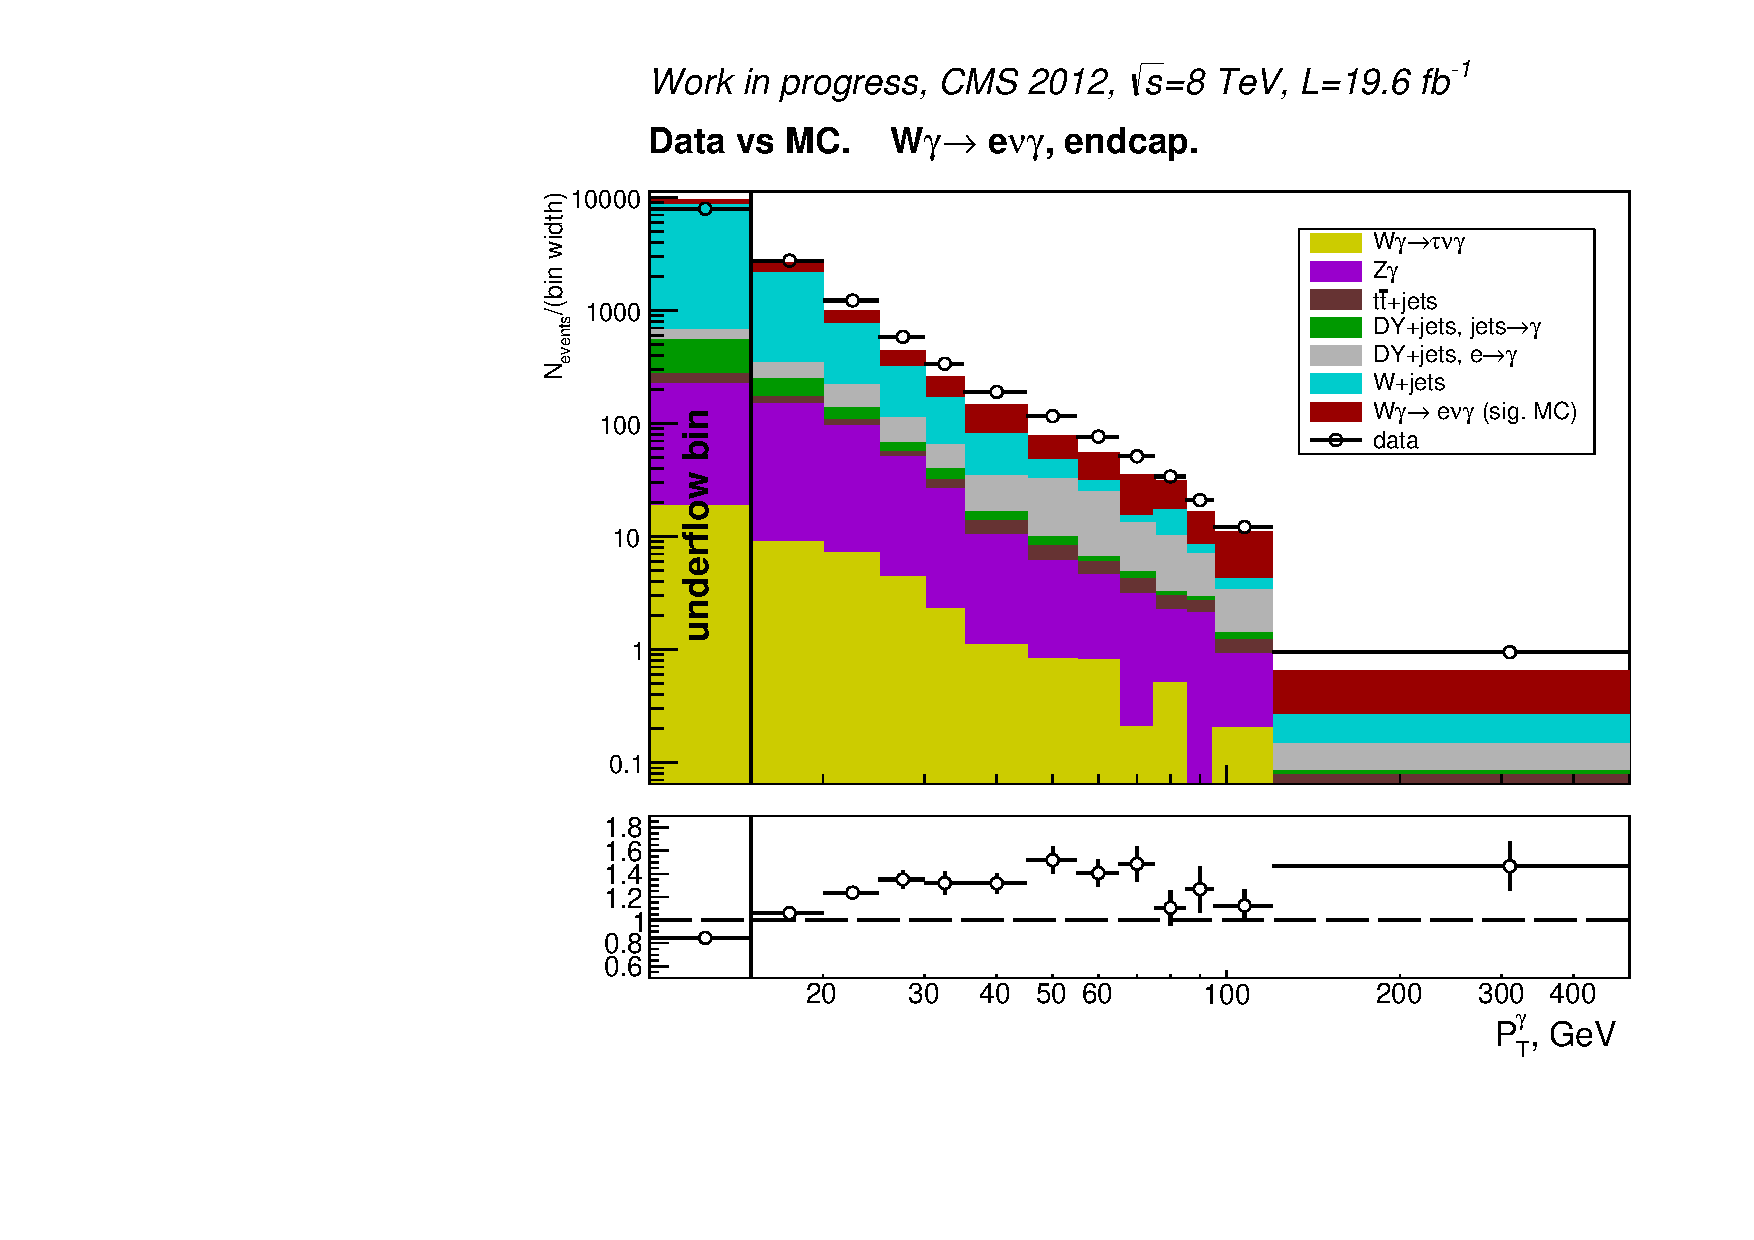
\includegraphics[width=0.45\textwidth]{../figs/figs_v11/ELECTRON_WGamma/PrepareYields/c_TotalDATAvsMC_Endcap__phoEt.pdf}
  \caption{$P_T^{\gamma}$ distribution of $W\gamma$ candidates. Data vs MC plots. Left column: muon channel, right column: electron channel. Top to bottom: photons in EB and EE of ECal.}
  \label{fig:DATAvsMC}
  \end{center}
\end{figure}
